\documentclass[a4paper, 11pt]{article}
\usepackage{comment} 
\usepackage{fullpage}
\usepackage{amsmath} 
\usepackage{amssymb} 
\usepackage{mathtools}
\usepackage{fontspec}
\defaultfontfeatures{Ligatures=TeX}
\usepackage{xfrac}
\usepackage{icomma}
\usepackage[section,below]{placeins}
\usepackage[labelfont=bf,font=small,width=0.9\textwidth]{caption}
\usepackage{subcaption}
\usepackage{graphicx}
\usepackage{grffile}
\usepackage{float}
\floatplacement{figure}{htbp}
\floatplacement{table}{htbp}
\usepackage{booktabs}
\usepackage{hyperref}
\usepackage[ngerman]{babel}
\usepackage{pdfpages}

\begin{document}
\noindent
%\centerline{\small{\textsc{Technische Universität Dortmund}}} \\
\large{\textbf{10. Übungsblatt zur Vorlesung \hfill WS 2017/2018 \\
Statistische Methoden der Datenanalyse \hfill Prof. W. Rhode}} \\
Annika Burkowitz, Sebastian Bange, Alexander Harnisch \\
\noindent\makebox[\linewidth]{\rule{\textwidth}{0.4pt}}

\section*{Aufgabe 31}
Die Variablennamen im Code richten sich alle nach der Vorlesung, wegen der fehlenden Kommentare sei daher auf diese verwiesen. Das zu fittende Polynom hat die Form \textit{test}
\begin{equation}
    p(x) = a_0 + a_1x + a_2x^2 + a_3x^3 + a_4x^4 + a_5x^5 + a_6x^6\,.
    \label{eqn:poly}
\end{equation}

\subsection*{a)}
Für die Koeffizienten erhalten wir
\begin{equation}
    \begin{split}
        a_0 &= -6,74453270\cdot 10^{-2} \\
        a_1 &= 6,09609038\cdot 10^{-1}  \\
        a_2 &= -5,13748213\cdot 10^{-1} \\
        a_3 &= 2,10566521\cdot 10^{-1}  \\
        a_4 &= -4,52007751\cdot 10^{-2} \\
        a_5 &= 4,78568049e\cdot 10^{-3}  \\
        a_6 &= -1,96288196e\cdot 10^{-4}\,. \\
    \end{split}
\end{equation}
Das Ergebnis ist in Abbildung~\ref{fig:31a} dargestellt.
\begin{figure}
    \centering
    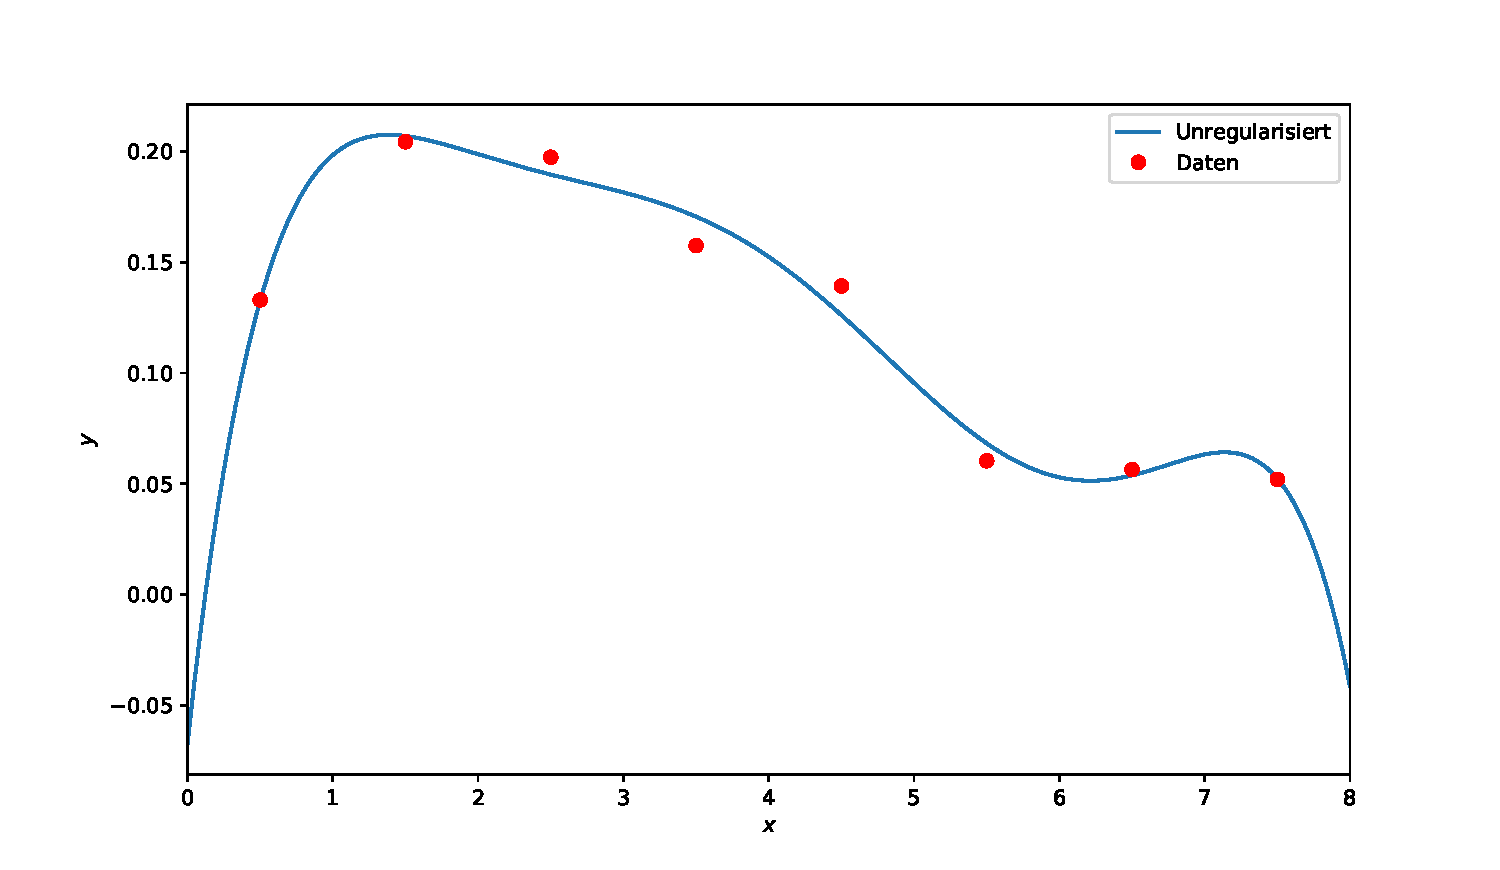
\includegraphics[width=\textwidth]{../A31/A31a.pdf}
    \caption{Geringste Quadrate Fit ohne Regularisierung an die Daten \textit{aufg\_a.csv}.}
    \label{fig:31a}
\end{figure}
\FloatBarrier

\subsection*{b)}
Falls ihr die Koeffizienten wirklich vergleichen wollt, werden diese vom Skript ausgegeben. Das Ergebnis ist in Abbildung~\ref{fig:31b} dargestellt.
\begin{figure}
    \centering
    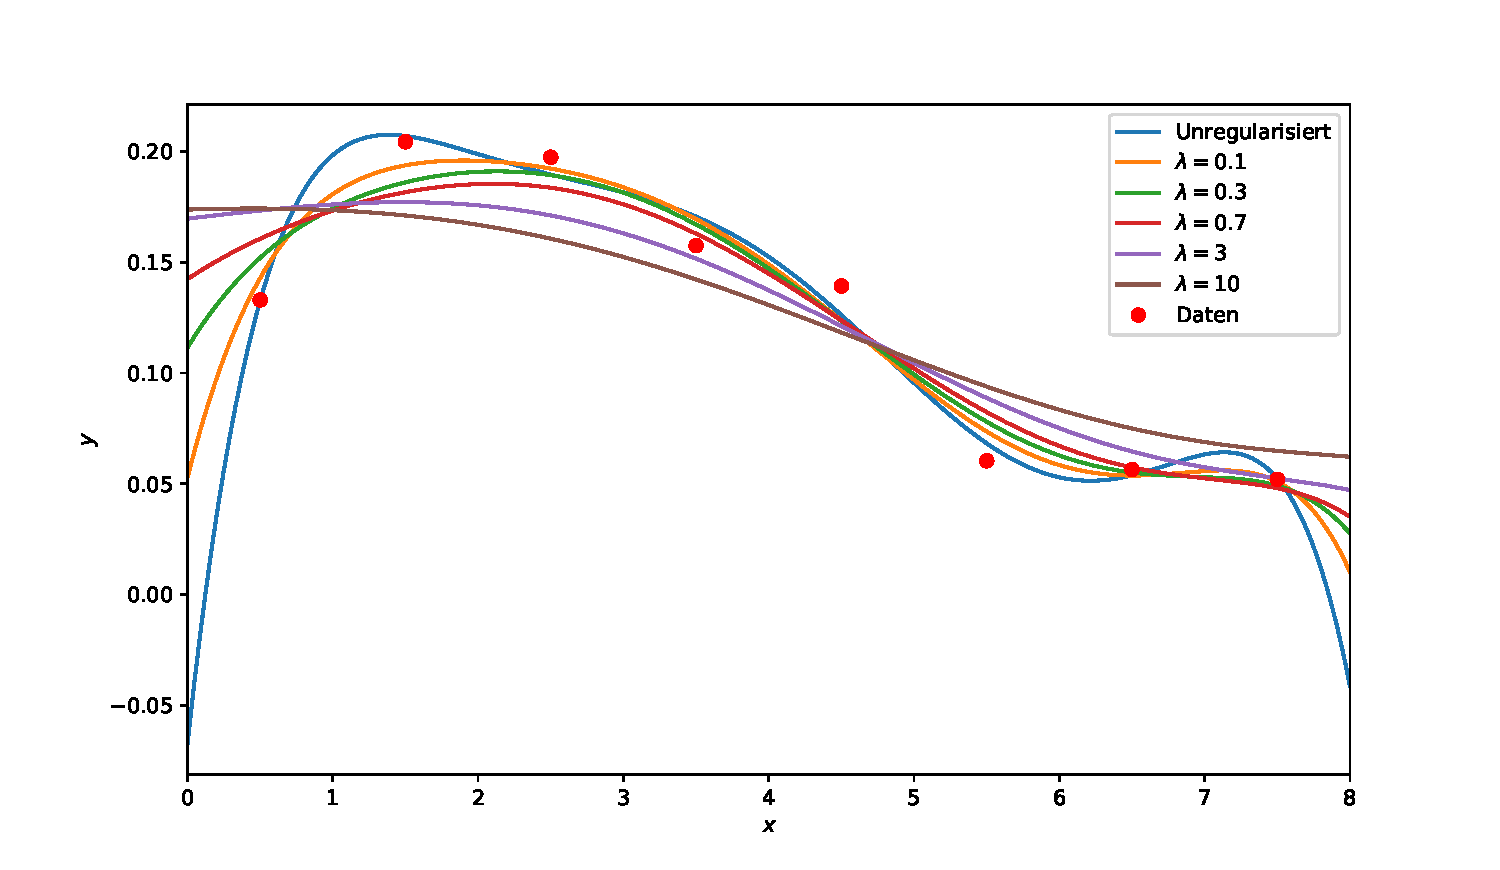
\includegraphics[width=\textwidth]{../A31/A31b.pdf}
    \caption{Geringste Quadrate Fit mit Regularisierung durch die zweite Ableitung für verschiedene Regularisierungsstärken $\lambda$ an die Daten \textit{aufg\_a.csv}.}
    \label{fig:31b}
\end{figure}
\FloatBarrier

\subsection*{c)}
Das Ergebnis ist in Abbildung~\ref{fig:31c} dargestellt.
\begin{figure}
    \centering
    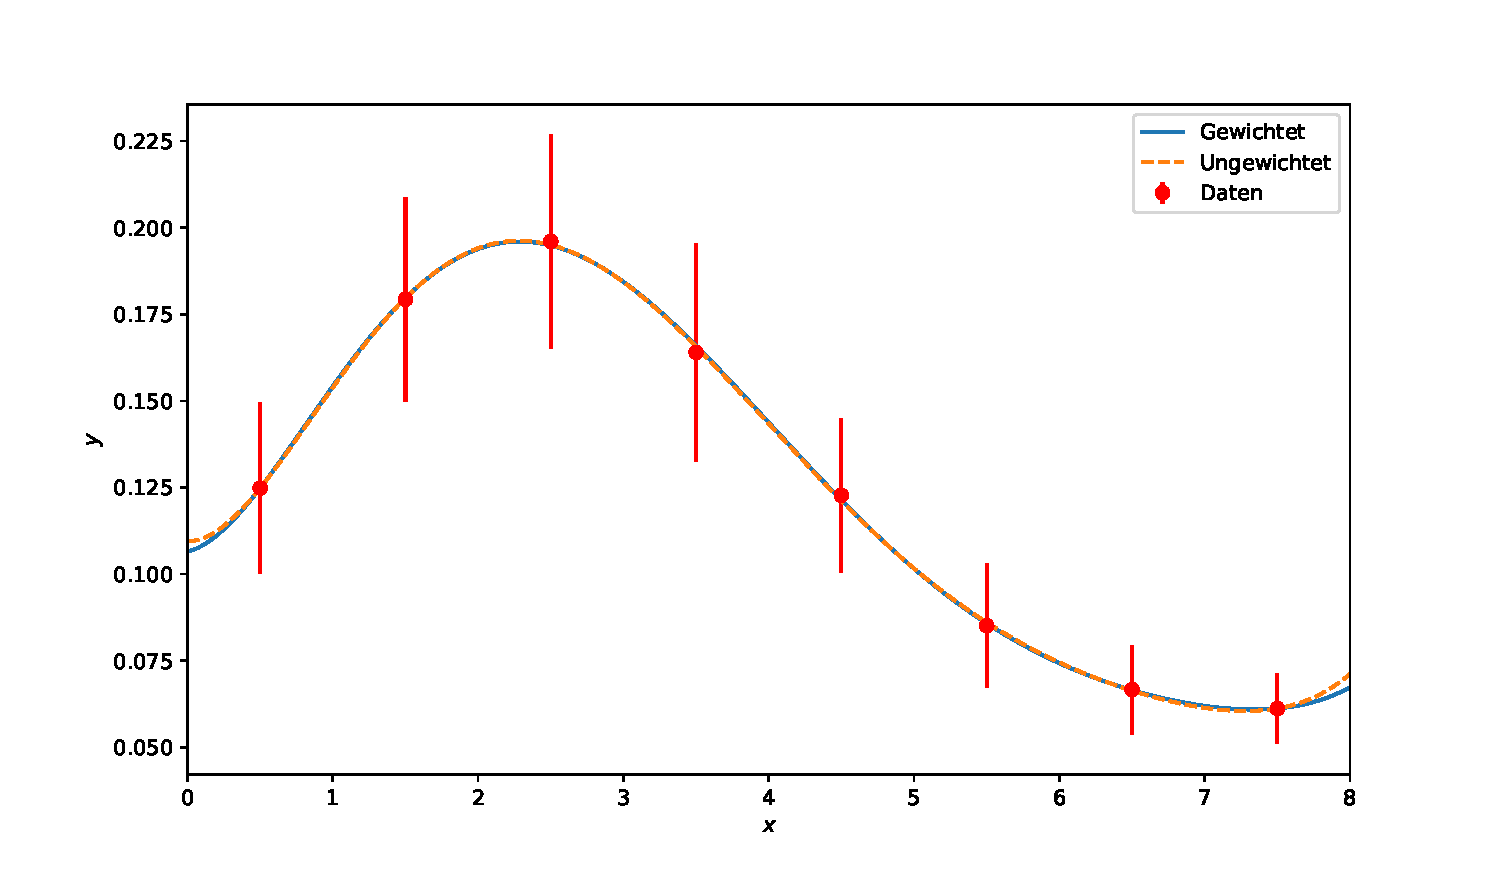
\includegraphics[width=\textwidth]{../A31/A31c.pdf}
    \caption{Gewichteter geringste Quadrate Fit ohne Regularisierung an die Daten \textit{aufg\_c.csv}.}
    \label{fig:31c}
\end{figure}
\FloatBarrier

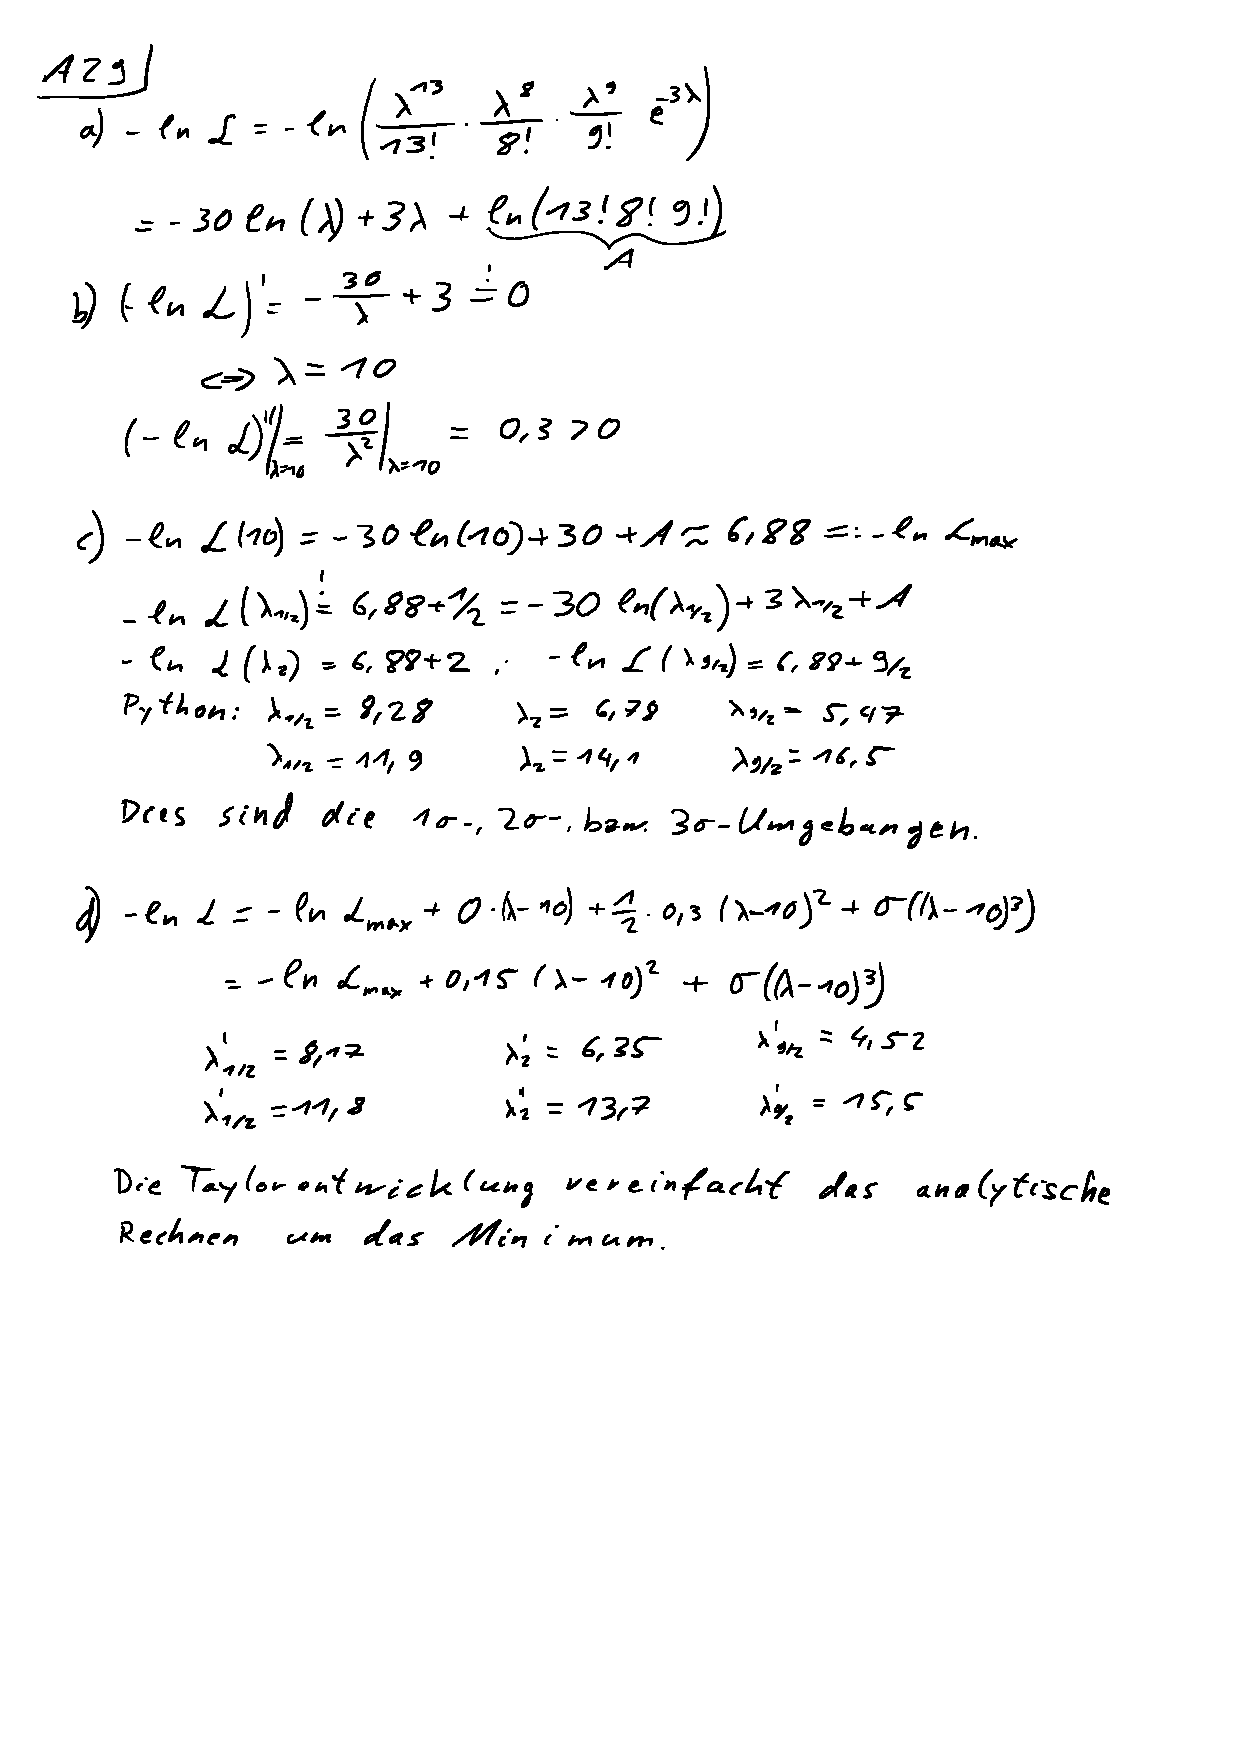
\includepdf[pages=1]{../Rechnungen.pdf}
\FloatBarrier
\begin{figure}
    \centering
    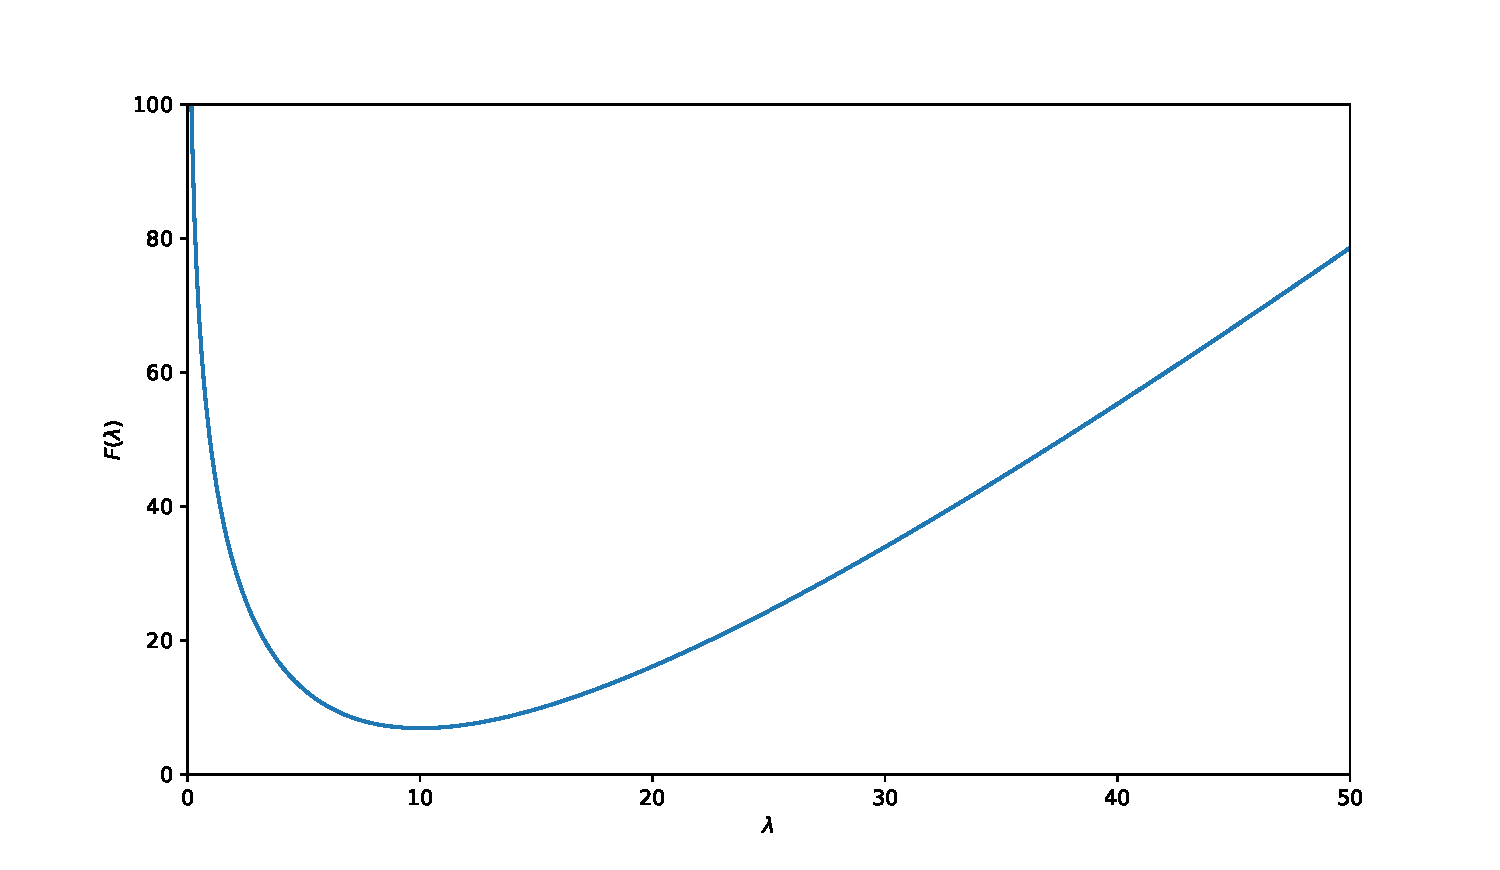
\includegraphics[width=\textwidth]{../A29/A29a.pdf}
    \caption{Negative Log-Likelihood-Funktion.}
\end{figure}
\begin{figure}
    \centering
    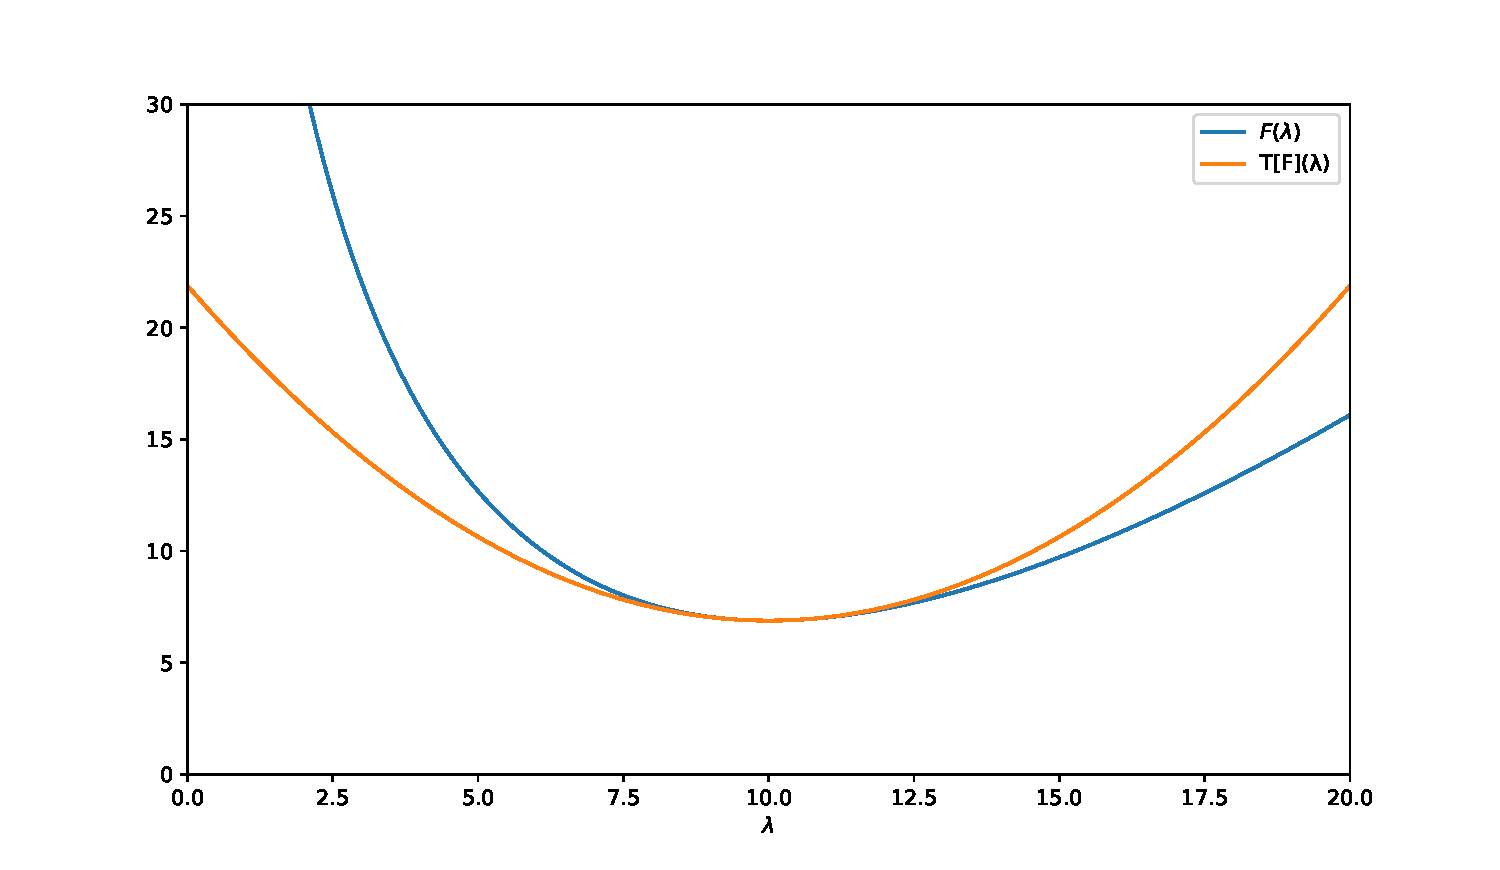
\includegraphics[width=\textwidth]{../A29/A29d.pdf}
    \caption{Negative Log-Likelihood-Funktion, zusammen mit der Taylorentwicklung um das Minimum.}
\end{figure}
\FloatBarrier

\includepdf[pages=2-3]{../Rechnungen.pdf}

\end{document}